\section*{Mutual Inductance} \label{sec:Mutual Inductance}
	\subsection*{Equivalent Mutual Inductance}
		\begin{table}[h!] % Mutual Inductance Equivalency Table
			\centering
			\renewcommand{\arraystretch}{2.25}
			\begin{tabular}{|c|c|c|}
			\hline
			Series-\textbf{Aiding} Connection & $L=L_{1}+L_{2}+2M$ & 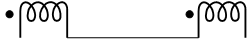
\includegraphics[scale=0.35]{Mutual_Inductors_Series_Dots_Aiding.png} \\ \hline
			Series-\textbf{Opposing} Connection & $L=L_{1}+L_{2}-2M$ & 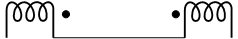
\includegraphics[scale=0.35]{Mutual_Inductors_Series_Dots_Opposing.png} \\ \hline
			\end{tabular}
		\end{table}

	\subsection*{Dot Convention} \label{subsec:Dot Convention}
		There are 2 cases:
		\begin{enumerate}[noitemsep, nolistsep]
			\item Current enters through dotted side on 1 inductor $\longrightarrow$ \textbf{POSITIVE VOLTAGE ON DOTTED SIDE OF OTHER INDUCTOR}
				\begin{itemize}[noitemsep, nolistsep]
					\item Current flows into the dotted side of one inductor
					\item Current flows out of the un-dotted side of second inductor, just like the first
				\end{itemize}
			\item Current enters through \textbf{NON}-dotted side of 1 inductor $\longrightarrow$ \textbf{POSITIVE VOLTAGE ON UN-DOTTED SIDE OF OTHER INDUCTOR}
				\begin{itemize}[noitemsep, nolistsep]
					\item Current flows into the un-dotted side of one inductor
					\item Current flows out of the dotted side of the second inductor, just like the first
				\end{itemize}
		\end{enumerate}
	
	\subsection*{Solving Disjoint Coupled Circuits} \label{subsec:Solve Disjoint Coupled Circuits}
		\begin{enumerate}[noitemsep] % Steps
			\item Apply KVL
			\item Don't forget about the Mutual Inductance Voltage Difference because of the first current
			\item There is a second way to thing about these, shown in Figures~\ref{subfig:Disjoint Coupled Inductors OG}~and~\ref{subfig:Disjoint Coupled Inductors Simplified}, below.
		\end{enumerate}
		\begin{figure}[ht!] % Convert
			\begin{subfigure}{0.5\textwidth}
				\centering
				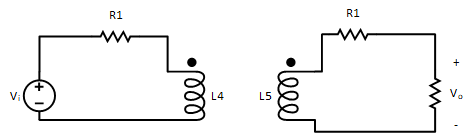
\includegraphics[scale=0.35]{Disjoint_Coupled_Inductors-OG.png}
				\subcaption{Original Circuit}
				\label{subfig:Disjoint Coupled Inductors OG}
			\end{subfigure}
			\begin{subfigure}{0.5\textwidth}
				\centering
				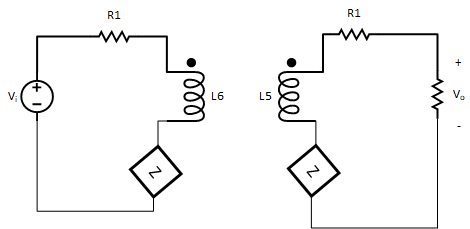
\includegraphics[scale=0.30]{Disjoint_Coupled_Inductors-Simplified.png}
				\subcaption{Circuit "Simplified" by Adding Dependent Sources}
				\label{subfig:Disjoint Coupled Inductors Simplified}
			\end{subfigure}
		\end{figure}
		\textbf{The sign on the dependent sources depends on which side of the inductor the current is going into.} \newline
		\textbf{Use the \nameref{subsec:Dot Convention} to determine which direction the source's voltage should go.}
	\vspace{-6mm}